%% BioMed_Central_Tex_Template_v1.06
%%                                      %
%  bmc_article.tex            ver: 1.06 %
%                                       %

%%IMPORTANT: do not delete the first line of this template
%%It must be present to enable the BMC Submission system to
%%recognise this template!!

%%%%%%%%%%%%%%%%%%%%%%%%%%%%%%%%%%%%%%%%%
%%                                     %%
%%  LaTeX template for BioMed Central  %%
%%     journal article submissions     %%
%%                                     %%
%%          <8 June 2012>              %%
%%                                     %%
%%                                     %%
%%%%%%%%%%%%%%%%%%%%%%%%%%%%%%%%%%%%%%%%%


%%%%%%%%%%%%%%%%%%%%%%%%%%%%%%%%%%%%%%%%%%%%%%%%%%%%%%%%%%%%%%%%%%%%%
%%                                                                 %%
%% For instructions on how to fill out this Tex template           %%
%% document please refer to Readme.html and the instructions for   %%
%% authors page on the biomed central website                      %%
%% http://www.biomedcentral.com/info/authors/                      %%
%%                                                                 %%
%% Please do not use \input{...} to include other tex files.       %%
%% Submit your LaTeX manuscript as one .tex document.              %%
%%                                                                 %%
%% All additional figures and files should be attached             %%
%% separately and not embedded in the \TeX\ document itself.       %%
%%                                                                 %%
%% BioMed Central currently use the MikTex distribution of         %%
%% TeX for Windows) of TeX and LaTeX.  This is available from      %%
%% http://www.miktex.org                                           %%
%%                                                                 %%
%%%%%%%%%%%%%%%%%%%%%%%%%%%%%%%%%%%%%%%%%%%%%%%%%%%%%%%%%%%%%%%%%%%%%

%%% additional documentclass options:
%  [doublespacing]
%  [linenumbers]   - put the line numbers on margins

%%% loading packages, author definitions

%\documentclass[twocolumn]{bmcart}% uncomment this for twocolumn layout and comment line below
\documentclass{bmcart}

%%% PACKAGES

\usepackage{xr}
\externaldocument{supplement}

\usepackage{booktabs} % for much better looking tables
\usepackage{array} % for better arrays (eg matrices) in maths
% \usepackage{paralist} % very flexible & customisable lists (eg. enumerate/itemize, etc.)
%   \let\itemize\compactitem
%   \let\enditemize\endcompactitem
%   \let\enumerate\compactenum
%   \let\endenumerate\endcompactenum
%   \let\description\compactdesc
%   \let\enddescription\endcompactdesc
%   \pltopsep=1pt
%   \plitemsep=1pt
%   \plparsep=1pt
\usepackage{hyperref}
\usepackage{xspace}
%\usepackage{geometry}
\usepackage{amsmath,amssymb}
\usepackage{bm}
\usepackage{verbatim}
\usepackage{longtable}
\usepackage[vlined]{algorithm2e}

\usepackage{inconsolata}

\usepackage{xifthen}
\usepackage{stmaryrd}

\usepackage{xcolor}

\usepackage{todonotes}


\hypersetup{
    bookmarks=false,         % show bookmarks bar?
    unicode=false,          % non-Latin characters in Acrobat’s bookmarks
    pdftoolbar=true,        % show Acrobat’s toolbar?
    pdfmenubar=true,        % show Acrobat’s menu?
    pdffitwindow=true,     % window fit to page when opened
    pdfstartview={FitH},    % fits the width of the page to the window
    colorlinks=true,       % false: boxed links; true: colored links
%    linkcolor=red!70!black,          % color of internal links (change box color with linkbordercolor)
%    citecolor=red!70!black,        % color of links to bibliography
    linkcolor=black,          % color of internal links (change box color with linkbordercolor)
    citecolor=black,        % color of links to bibliography
    filecolor=magenta,      % color of file links
    urlcolor=red!70!black           % color of external links
}



%%%%%%%%%%%%%%%%%%%%%%%%%%%%%%%%%%%%%%%%%%%%%%%%%
%%                                             %%
%%  If you wish to display your graphics for   %%
%%  your own use using includegraphic or       %%
%%  includegraphics, then comment out the      %%
%%  following two lines of code.               %%
%%  NB: These line *must* be included when     %%
%%  submitting to BMC.                         %%
%%  All figure files must be submitted as      %%
%%  separate graphics through the BMC          %%
%%  submission process, not included in the    %%
%%  submitted article.                         %%
%%                                             %%
%%%%%%%%%%%%%%%%%%%%%%%%%%%%%%%%%%%%%%%%%%%%%%%%%

%TODO uncomment
%\def\includegraphic{}
%\def\includegraphics{}



%%% Put your definitions there:
\startlocaldefs
%%%%%%%%%%%%%%%%%%%%%%%%%%%%%%%%%%%%%%%%
%% Rolf's includegraphicstop
\makeatletter
\newsavebox{\@alignepsbox}
\newlength{\@aligneps}
\newcommand{\includegraphicstop}[2][]{%
\sbox{\@alignepsbox}{\includegraphics[#1]{#2}}%
\setlength{\@aligneps}{-\ht\@alignepsbox}%
\addtolength{\@aligneps}{2ex}%
\raisebox{\@aligneps}{\usebox{\@alignepsbox}}}
\makeatother


%\makeatletter
%\let\oldlt\longtable
%\let\endoldlt\endlongtable
%\def\longtable{\@ifnextchar[\longtable@i \longtable@ii}
%\def\longtable@i[#1]{\begin{figure}[t]
%\onecolumn
%\begin{minipage}{0.5\textwidth}
%\oldlt[#1]
%}
%\def\longtable@ii{\begin{figure}[t]
%\onecolumn
%\begin{minipage}{0.5\textwidth}
%\oldlt
%}
%\def\endlongtable{\endoldlt
%\end{minipage}
%\twocolumn
%\end{figure}}
%\makeatother

%%%%%%%%%%%%%%%%% Theorems %%%%%%%%%%%%%%%%%%%%%%%%%

\newtheorem{theorem}{Theorem}
\newtheorem{definition}[theorem]{Definition}
\newtheorem{remark}[theorem]{Remark}
\newtheorem{corollary}[theorem]{Corollary}
\newtheorem{lemma}[theorem]{Lemma}
\newtheorem{proposition}[theorem]{Proposition}

\newtheorem{observation}[theorem]{Observation}

%\newtheorem{algorithm}{Algorithm}
\newtheorem{axiom}{Axiom}
\newtheorem{hypothesis}{Working Hypothesis}
\newenvironment{proof}[1][]{\noindent \em Proof\ifthenelse{\equal{#1}{}}{}{ (#1)}:~}{}

%%% macros for notation in DP framework
\newcommand{\network}{\mathcal{N}}
\newcommand{\val}{\bar S} % valuation aka assignment
\newcommand{\dep}{\operatorname{dep}}
\newcommand{\energy}[1]{\operatorname{e}_{#1}}
\newcommand{\numberof}{\operatorname{\#}}
\newcommand{\partfun}[1]{Z_{#1}}
\newcommand{\separator}[2]{\operatorname{sep}(#1,#2)}
\newcommand{\difference}[2]{\operatorname{diff}(#1 \rightarrow #2)}
\newcommand{\real}{\mathbb{R}}
\newcommand{\genmarg}[1]{(\!|\!#1\!|\!)}
\newcommand{\gencomb}[1]{\langle\!|#1|\!\rangle}
\newcommand{\Message}[2]{m_{#1\rightarrow #2}}


\newcommand{\energyModel}{{\cal M}}
\newcommand{\structureElements}{{\cal SE}}
\newcommand{\powerSet}[1]{2^{#1}}
\newcommand{\underConstruction}[1]{{\LARGE$\triangle$\Large\!\!\!\!!}$\quad$\textcolor{red}{#1}}
\newcommand{\argmin}{\operatorname*{arg\,min}}
\newcommand{\objective}{{\mathbb{F}}}

\newcommand{\partseqs}{\mathcal{P\!S}}
\newcommand{\B}{\mathcal{B}}
\newcommand{\F}{\mathcal{F}}
\newcommand{\I}{\mathcal{I}}
\newcommand{\R}{\mathcal{R}}
\renewcommand{\S}{\mathcal{S}}
\newcommand{\X}{\mathcal{X}}
\newcommand{\Y}{\mathcal{Y}}

\newcommand{\width}{w}

\newcommand{\sample}{\texttt{Sample}}
\newcommand{\elim}[2]{\operatorname{elim}(#1,#2)}

%\newcommand{\Ehp}[1]{E^{\textrm{hp}}(#1)}
%\newcommand{\Eint}[1]{E^{\textrm{int}}(#1)}

\newcommand{\EbpSym}{E^{\textrm{bp}}}
\newcommand{\Ebp}[2]{\EbpSym_{#1}(#2)}

\newcommand{\Def}[1]{\emph{#1}}

\newcommand{\TargetE}{E^{\star}}
%\newcommand{\MFE}{\text{\rm MFE}}
\newcommand{\EnsE}{\text{\rm G}} %ensemble energy

\newcommand{\Obj}{\text{\rm MultiDefect}}

\newcommand{\TODO}[1]{\textcolor{red!70!black}{\textbf{TODO: #1}}}

\newcommand{\parHead}[1]{\Final{\paragraph{#1}}}

\newcommand{\Final}[1]{\begingroup\color{red!70!black}#1\endgroup}
%% Uncomment the line below for ``Final'' version
\renewcommand{\Final}[1]{}

\newcommand{\Design}[1]{{\sf Designs}^{\star}(#1)}
\newcommand{\NumDesign}{\ensuremath{\#}{\sf Designs}\xspace}
\newcommand{\IS}[1]{{\sf IndSets}(#1)}
\newcommand{\Nuc}[1]{{\sf #1}}
\newcommand{\Ab}{\Nuc{A}}
\newcommand{\Cb}{\Nuc{C}}
\newcommand{\Gb}{\Nuc{G}}
\newcommand{\Ub}{\Nuc{U}}

\newcommand{\Objectiv}{\Nuc{U}}


\newcommand{\GCb}{\Gb\Cb}

\newcommand{\Software}[1]{{\ttfamily #1}}

\newcommand{\substitute}[2]{#1\!\oplus\!#2}
%\newcommand{\evalfor}[2]{#1\llbracket{}#2\rrbracket{}}
\newcommand{\evalfor}[2]{#1(#2)}

\renewcommand{\gets}{:=}

\setlength{\parskip}{.2em}

\newcommand{\RNAblueprint}{{\tt \bfseries{}\color{black!85} RNA\textcolor{blue!70!black}{Blue}Print}}
\newcommand{\ourprog}{{\tt \bfseries{}\color{black!85}RNA\textcolor{red!70!black}{Red}Print}}

\newcommand{\Energy}[2]{E(#2;#1)}

\newcommand{\EnergyTurner}{E_{\text{T}}}
\newcommand{\EnergyStacking}{E_{\text{st}}}

\newcommand{\citep}[1]{\cite{#1}}
\newcommand{\citet}[1]{\cite{#1}}

%%% end macro defs

%% fix some weirdness of the bioinfo class (footer overlapping text on page 1)
\makeatletter
\setlength\footskip{30\p@}          % space above footer line
\makeatother

\endlocaldefs

%%% Begin ...
\begin{document}


%%% Start of article front matter
\begin{frontmatter}

\begin{fmbox}
\dochead{Research}

%%%%%%%%%%%%%%%%%%%%%%%%%%%%%%%%%%%%%%%%%%%%%%
%%                                          %%
%% Enter the title of your article here     %%
%%                                          %%
%%%%%%%%%%%%%%%%%%%%%%%%%%%%%%%%%%%%%%%%%%%%%%

%[Efficient Sampling for Multi-Target RNA Design]
\title{Fixed-Parameter Tractable Sampling for RNA Design with Multiple Target Structures}


%%%%%%%%%%%%%%%%%%%%%%%%%%%%%%%%%%%%%%%%%%%%%%
%%                                          %%
%% Enter the authors here                   %%
%%                                          %%
%% Specify information, if available,       %%
%% in the form:                             %%
%%   <key>={<id1>,<id2>}                    %%
%%   <key>=                                 %%
%% Comment or delete the keys which are     %%
%% not used. Repeat \author command as much %%
%% as required.                             %%
%%                                          %%
%%%%%%%%%%%%%%%%%%%%%%%%%%%%%%%%%%%%%%%%%%%%%%

% \author[Hammer, Ponty, Wang and Will]{Stefan Hammer\,$^{\text{\sfb 1,2,3}}$, Yann Ponty\,$^{\text{\sfb 4,5,}\star}$, Wei Wang\,$^{\text{\sfb 4}}$ and Sebastian Will\,$^{\text{\sfb 2}}$}

\author[
    addressref={aff1,aff2,aff3},
    email={stefan.hammer@uni-leipzig.de}
]{\inits{F}\fnm{Stefan} \snm{Hammer}}
%
\author[
    addressref={aff4,aff5},
    corref={aff4},                       % id of corresponding address, if any
    email={yann.ponty@lix.polytechnique.fr}
]{\inits{F}\fnm{Yann} \snm{Ponty}}
%
\author[
    addressref={aff4},
    email={wei.wang@lix.polytechnique.fr}
]{\inits{F}\fnm{Wei} \snm{Wang}}
%
\author[
    addressref={aff2,aff3},
    %corref={aff2},                       % id of corresponding address, if any
    email={will@tbi.univie.ac.at}
]{\inits{S}\fnm{Sebastian} \snm{Will}}


%%%%%%%%%%%%%%%%%%%%%%%%%%%%%%%%%%%%%%%%%%%%%%
%%                                          %%
%% Enter the authors' addresses here        %%
%%                                          %%
%% Repeat \address commands as much as      %%
%% required.                                %%
%%                                          %%
%%%%%%%%%%%%%%%%%%%%%%%%%%%%%%%%%%%%%%%%%%%%%%


% \address{$^{\text{\sf 1}}$University Leipzig, Department of Computer Science and Interdisciplinary Center for Bioinformatics, 04107 Leipzig, Germany;
\address[id=aff1]{%                           % unique id
  \orgname{Dept.\ Computer Science, and Interdisciplinary Center
      for Bioinformatics, Univ.\ Leipzig}, 
  \street{H{\"a}rtelstr.\ 16-18},                     
  \postcode{D-04107},   
  \city{Leipzig}, 
  \cny{Germany}  
}

% $^{\text{\sf 2}}$University of Vienna, Faculty of Chemistry, Department of Theoretical Chemistry, 1090 Vienna, Austria;
\address[id=aff2]{%
    \orgname{Dept.\ Theoretical Chemistry, Univ.\ Vienna},
    \street{W{\"a}hringerstr.\ 17},
    \postcode{A-1090}
    \city{Wien},
    \cny{Austria}
}

% $^{\text{\sf 3}}$University of Vienna, Faculty of Computer Science, Research Group Bioinformatics and
% Computational Biology, 1090 Vienna, Austria;
\address[id=aff3]{%
    \orgname{Bioinformatics and Computational Biology Research Group, Univ.\ Vienna},
    \street{W{\"a}hringerstr.\ 17},
    \postcode{A-1090}
    \city{Wien},
    \cny{Austria}
}

% $^{\text{\sf 4}}$CNRS UMR 7161 LIX, Ecole Polytechnique, Bat. Turing, 91120 Palaiseau, France;
\address[id=aff4]{%
    \orgname{CNRS UMR 7161 LIX, Ecole Polytechnique},
    \street{Bat. Alan Turing},
    \postcode{91120}
    \city{Palaiseau},
    \cny{France}
}

% $^{\text{\sf 5}}$ AMIBio team, Inria Saclay, Bat Alan Turing, 91120 Palaiseau, France}
\address[id=aff5]{%
    \orgname{AMIBio team, Inria Saclay},
    \street{Bat. Alan Turing},
    \postcode{91120}
    \city{Palaiseau},
    \cny{France}
}


%%%%%%%%%%%%%%%%%%%%%%%%%%%%%%%%%%%%%%%%%%%%%%
%%                                          %%
%% Enter short notes here                   %%
%%                                          %%
%% Short notes will be after addresses      %%
%% on first page.                           %%
%%                                          %%
%%%%%%%%%%%%%%%%%%%%%%%%%%%%%%%%%%%%%%%%%%%%%%

\begin{artnotes}
%\note{Sample of title note}     % note to the article
%\note[id=n1]{Equal contributor} % note, connected to author
\end{artnotes}

\end{fmbox}% comment this for two column layout

%%%%%%%%%%%%%%%%%%%%%%%%%%%%%%%%%%%%%%%%%%%%%%
%%                                          %%
%% The Abstract begins here                 %%
%%                                          %%
%% Please refer to the Instructions for     %%
%% authors on http://www.biomedcentral.com  %%
%% and include the section headings         %%
%% accordingly for your article type.       %%
%%                                          %%
%%%%%%%%%%%%%%%%%%%%%%%%%%%%%%%%%%%%%%%%%%%%%%

\begin{abstractbox}
\begin{abstract}
  \parttitle{Background}
  The design of multi-stable RNA molecules has important applications in biology, medicine, and biotechnology. Synthetic design approaches profit strongly from effective in-silico methods, which can tremendously impact their cost and feasibility. \\
  \parttitle{Results} We revisit a central ingredient of most in-silico
  design methods: the sampling of sequences for the design of
  multi-target structures, possibly including pseudoknots. For this
  task, we present the efficient, tree decomposition-based algorithm
  \ourprog{}. Our fixed parameter tractable approach is underpinned by
  establishing the $\#${\sf P}-hardness of uniform sampling. Modeling
  the problem as a constraint network, \ourprog{} supports generic
  Boltzmann-weighted sampling for arbitrary additive RNA energy
  models; this enables the generation of RNA sequences meeting
  specific goals like expected free energies or \GCb-content. Finally,
  we empirically study general properties of the approach and generate
  biologically relevant multi-target Boltzmann-weighted designs for a
  common design benchmark, including pseudoknots. Generating seed sequences with \ourprog{}, we demonstrate significant improvements over the previously best multi-target sampling strategy.\\
  

  \smallskip
  \noindent
  Our free software is available at: \url{https://github.com/yannponty/RNARedPrint}\\
  Supplementary data are available online.
\end{abstract}

%%%%%%%%%%%%%%%%%%%%%%%%%%%%%%%%%%%%%%%%%%%%%%
%%                                          %%
%% The keywords begin here                  %%
%%                                          %%
%% Put each keyword in separate \kwd{}.     %%
%%                                          %%
%%%%%%%%%%%%%%%%%%%%%%%%%%%%%%%%%%%%%%%%%%%%%%

\begin{keyword}
  \kwd{RNA multi-target design}
  \kwd{RNA secondary structure}
  \kwd{Multi-dimensional Boltzmann sampling}
  \kwd{{$\#$}{\sf P}-hardness of RNA design}
\end{keyword}

% MSC classifications codes, if any
%\begin{keyword}[class=AMS]
%\kwd[Primary ]{}
%\kwd{}
%\kwd[; secondary ]{}
%\end{keyword}

\end{abstractbox}
%
%\end{fmbox}% uncomment this for twcolumn layout

\end{frontmatter}

%%%%%%%%%%%%%%%%%%%%%%%%%%%%%%%%%%%%%%%%%%%%%%
%%                                          %%
%% The Main Body begins here                %%
%%                                          %%
%% Please refer to the instructions for     %%
%% authors on:                              %%
%% http://www.biomedcentral.com/info/authors%%
%% and include the section headings         %%
%% accordingly for your article type.       %%
%%                                          %%
%% See the Results and Discussion section   %%
%% for details on how to create sub-sections%%
%%                                          %%
%% use \cite{...} to cite references        %%
%%  \cite{koon} and                         %%
%%  \cite{oreg,khar,zvai,xjon,schn,pond}    %%
%%  \nocite{smith,marg,hunn,advi,koha,mouse}%%
%%                                          %%
%%%%%%%%%%%%%%%%%%%%%%%%%%%%%%%%%%%%%%%%%%%%%%

%%%%%%%%%%%%%%%%%%%%%%%%% start of article main body
% <put your article body there>

%%%%%%%%%%%%%%%%
%% Background %%
%%
\section*{Background}
\parHead{Design, applications and motivation for multiple design.}Synthetic biology endeavors the engineering of artificial biological
systems, promising broad applications in biology, biotechnology and
medicine. Centrally, this requires the design of biological
macromolecules with highly specific properties and programmable functions.
RNA present itself as a well-suited tool for a
rational design targeting specific functions~\citep{Kushwaha2016}. RNA function is tightly
coupled to the formation of secondary structure, as well as changes in
base pairing propensities and the accessibility of regions, e.g.\ by
burying or exposing interaction sites~\citep{Rodrigo2014}. At the same time, the
thermodynamics of RNA secondary structure is well understood and its prediction is
computationally tractable~\citep{McCaskill1990}. Thus,  structure can serve as effective
proxy for rational design approaches, ultimately targeting catalytic~\citep{Zhang2013} or regulatory functions.

\parHead{Motivating multiple RNA design.} The function of many RNAs
depends on their selective folding into one or several alternative
conformations. Classic examples include riboswitches, which
notoriously adopt different stable structures upon binding a specific
ligand. Riboswitches have been a popular application of rational
design~\citep{Wachsmuth2013,Domin2017}, partly motivated by their
capacity to act as biosensors~\citep{Findeiss2017}. At the
co-transcriptional level, certain RNA families feature alternative,
evolutionarily conserved, transient structures~\citep{Zhu2013}, which
facilitate the ultimate adoption of functional structures at full
elongation.  More generally, simultaneous compatibility to multiple
structures is a relevant design objective for engineering kinetically
controlled RNAs, finally targeting prescribed folding pathways. Thus,
modern applications of RNA design often target multiple structures,
additionally aiming at other features, such as specific
\GCb-content (\GCb\%) as previously done by~\citet{Reinharz2013} or the presence/absence of
functionally relevant motifs (either anywhere or at specific
positions)~\citep{Zhou2013}; these objectives motivate flexible
computational design methods.

\parHead{On the importance of sampling for design.}
Many computational methods for RNA design rely on similar overall
strategies: initially generating one or several \Def{seed} sequences
and optimizing them subsequently. In many cases, the seed quality was
found to be critical for the empirical performance of RNA design
methods~\citep{Levin2012}. For instance, random seed generation
improves the prospect of subsequent optimizations, helping to overcome
local optima of the objective function, and increases the diversity
across designs~\citep{Reinharz2013}.  For single-target approaches,
\Software{INFO-RNA}~\citep{Busch2006} made significant improvements
mainly by starting its local search from the minimum energy sequence
for the target structure instead of (uniform) random sequences for the
early \Software{RNAinverse} algorithm~\citep{Hofacker1994}. This
strategy was later shown to result in unrealistically high
\GCb\% in designed sequences. To address this issue,
tools like \Software{antaRNA}~\citep{Kleinkauf2015} and \Software{IncaRNAtion}~\citep{Reinharz2013} control \GCb\%; the latter based on adaptive sampling.

\parHead{Specificities and similarities of multi-target design.}
Specifically, for multi-target design, virtually all available methods~\citep{Lyngsoe2012,HoenerzuSiederdissen2013,Taneda2015,Hammer2017} follow the same overall generate-and-optimize strategy.
%
Facing the complex sequence constraints induced by multiple targets, early methods such as \Software{Frnakenstein}~\citep{Lyngsoe2012} and \Software{Modena}~\citep{Taneda2015} did not attempt to solve sequence generation systematically, but rely on ad-hoc sampling strategies.
%
Recently, the approach \Software{RNAdesign}~\citep{HoenerzuSiederdissen2013}, coupled with local
search within \RNAblueprint{}~\citep{Hammer2017}, solved the
problem of sampling seeds from the \emph{uniform} distribution for multiple
target structures. \Software{RNAdesign} adopts a graph coloring perspective,
coloring the sequence positions with nucleotides, such that the ends of each base pair receive compatible colors. Initially the method decomposes the graph hierarchically using ear decomposition, and then \Def{precomputes} the number of valid sequences
within each subgraph. The decomposition is then reinterpreted as a
decision tree to perform a \Def{stochastic backtrack}, inspired by
Ding and Lawrence~\citep{Ding2003}. Uniform sampling is achieved by
choosing individual nucleotide assignments with probabilities derived
from the subsolution counts. The overall complexity of
\Software{RNAdesign} grows like $\Theta(4^{\gamma})$, where the
parameter $\gamma$, while bounded only by the length of the designed RNA, is 
typically much lower, due to the decomposition strategy.

\parHead{Motivation.} 
While uniform sampling in \Software{RNAdesign}/\RNAblueprint{} turned out to be very successful,
the work on these tools gave no definitive answer on the \emph{complexity of uniform sampling for multi-target design}. On the one hand, time and space requirements grow exponential in the general case,
the decomposition strategy seems to allow practical applications.
Better understanding of the true complexity bounds is still highly relevant for the application of such methods, in particular for applications in more expressive settings (e.g. Boltzmann sampling as discussed in this work or sampling satisfying multiple additional constraints and properties). All such extensions are still bounded by the complexity of the multi-target uniform sampling problem, where counting of valid designs is the dominating step (since stochastic backtrack can be performed in linear time per sample).

Consequently, for elucidating the theoretical fundament of RNA design sampling, we first need to clarify, whether efficient approaches for counting could exist. In Section~\ref{sec:counting}, we show that there can not exists any efficient, polynomial time algorithm unless ${\sf P}={\sf NP}$. Our result relies on a surprising bijection (up to a trivial symmetry) between valid sequences and independent sets of a bipartite graph, being the object of recent breakthroughs in approximate counting complexity~\citep{Bulatov2013,Cai2016}.

As already indicated by \Software{RNAdesign}, the hardness of counting (and conjectured hardness of sampling), does still not rule out practically applicable algorithms for counting and sampling.
Addressing the following questions in more detail and generality led to the practical advances in this work, which extend the expressivity, flexibility, and performance of multi-structure design: \emph{How to sample, in a general way, from a Boltzmann distribution based on expressive energy models? How to enforce additional constraints, such as \GCb\%, complex sequence constraints, or the energy of individual structures?}

\begin{figure*}[t]
\begin{center}
    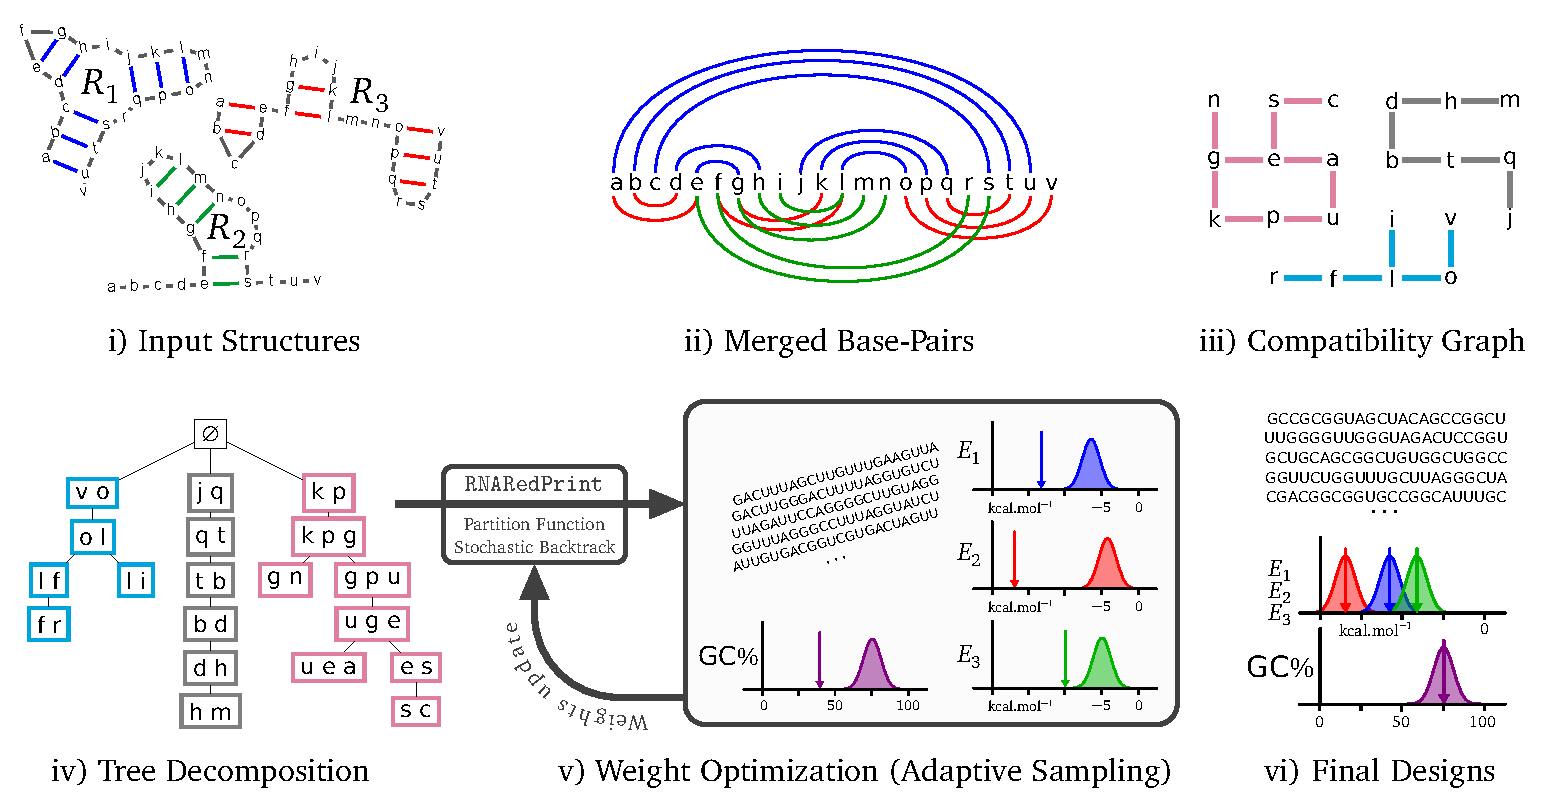
\includegraphics[width=.8\textwidth]{Workflow.pdf}
\end{center}
\caption{General outline of \ourprog{} for base pair-based energy models. From a set of target secondary structures (i), base-pairs are merged (ii) into a (base pair) dependency graph (iii) and transformed into a tree decomposition (iv). The tree is then used to compute the partition function, followed by a Boltzmann sampling of valid sequences (v). An adaptive scheme learns weights to achieve targeted energies and \GCb\%, leading to the production of suitable designs (vi).}
\label{fig:workflow}
\end{figure*}

To answer these questions, we introduce a generic framework (illustrated in~Fig.~\ref{fig:workflow}) enabling efficient Boltzmann-weighted sampling over RNA sequences with multiple target structures (Section~\ref{sec:FPT}). As main algorithmic contribution of this work, we devise a dynamic programming algorithm, based on a tree decomposition, to compute partition functions and sample sequences from the Boltzmann distribution%
% (Subsection~\ref{sec:PF})
. We show that these algorithms are \Def{fixed-parameter tractable (FPT)} for the \Def{treewidth},
in other words: they have polynomial time and space complexity for a fixed treewidth%
% Subsection~\ref{sec:complexity}
%
. Due to the generality of our method, we can moreover strongly limit this parameter in practice by using state-of-the-art tree decomposition algorithms.
%Uniform sampling is handled as a special case of Boltzmann sampling, where each valid sequence receives energy zero and---consequently---computing partition functions specializes to counting.
By evaluating (partial) sequences in a weighted constraint
network, we support arbitrary multi-ary constraints and thus
arbitrarily complex energy models,
notably subsuming all commonly
used RNA energy models%
%(Subsection~\ref{sec:energy_models})
.  Moreover, we describe an \Def{adaptive
  sampling} strategy to control the free energies of the individual
target structures and \GCb\%%
% (SubSection~\ref{sec:multiBoltzmann})
. %

We observe that
targeting realistic RNA energies in the realistic
Turner RNA energy model
works well by performing sampling based on less complex RNA energy models, which cause low treewidth. This result is highly relevant in practice, since it allows to combine high efficiency with high accuracy and moreover leaves room for extensions of the method.

Eventually this strategy allows generating biologically relevant
multi-target designs, as we demonstrate in our application 
to a large set of multi-target RNA design instances from a
representative benchmark (Section~\ref{sec:results}).

\section{Definitions and problem statement}
\label{sec:problem-statement}

An \Def{RNA sequence $S$} is a word over the \Def{nucleotides
  alphabet} $\Sigma=\{\Ab,\Cb,\Gb,\Ub\}.$
An \Def{RNA (secondary) structure $R$ of
  length $n$} is a set of \Def{base pairs} $(i,j)$, where
$1\leq i<j\leq n$, where for all different $(i,j), (i',j')\in R$:
$\{i,j\}\cap\{i',j'\}=\emptyset$ (``degree $\leq$ 1'').
%
% We call an RNA structure $R$ \Def{non-crossing}, iff it does not
% contain any two different base pairs $(i,j)$ and $(i',j')$ such that
% $i\leq i'\leq j \leq j'.$
%
\Def{Valid base pair} must pair bases from
$\B:=\left\{\{\Ab,\Ub\},\{\Gb,\Cb\},\{\Gb,\Ub\}\right\}.$
Consequently, $S$ is \Def{valid} for $R$, iff $\{S_i,S_j\}\in \B$ for
all $(i,j)\in R$.
 
RNA energy models like the Turner energy model~\citep{Turner2009} define an energy function that maps a pair of a sequence $S$ and a structure $R$ to a real value, the \Def{energy}. 
Typically, such energy functions are additively composed from energy contributions of structure elements (like single base pairs or loops). It is most instructive, and in this context already practically useful, to develop pour approach for the simple \Def{base pair energy model}. This model defines energy contributions $\EbpSym(x,y)$ for base pairs $(x,y)\in\Sigma^2$ that specify the energy function as
$
\EbpSym(S,R) = \sum_{(i,j)\in R} \EbpSym(S_i,S_j)
$
for each sequence $S\in\Sigma^n$ and structure $R$ for length $n$.

As the structural targets of our design, we fix the set of RNA structures
$\R:=\{R_1, \dots, R_k\}$ for sequences of length $n$.
Recall that we aim to generate random sequences that satisfy a number of constraints like the compatibility of paired bases. Moreover, we want to enforce that generated samples satisfy complex properties, which we express in terms of \emph{features}. An example of such a feature is the \GCb\% (the corresponding property of a sequence is to have a specific \GCb\%). The additional properties that we are going to enforce are specific 'target' energies for the single structures $R_1, \dots, R_k$; for this purpose, each such energy is considered as a feature.

Formally, we define a \Def{feature $F$} as function on sequences, which is expressed by summing over an associated set of \Def{feature functions} on sequences, such that
$$
F(S) = \sum_{\text{feature function $f$ associcated with $F$}} f(S).
$$
We emphasize that our approach is designed to profit (in terms of computational complexity) from feature functions that each depend only on few sequence positions. For example, the $\GCb\%$ feature is expressed by feature functions $f^{GC}_i$ where $f^{GC}_i(S)$ equals 1 if $S_i='G'$ or $S_i='C'$ and 0 otherwise. Similarly the base pair energy for a target structure $R$ is expressed as feature with feature functions $f^R_{ij}(S)=\EbpSym(S_i,S_j),$ such that $F(S)=\EbpSym(S,R)$. In both cases, the feature functions depend on the nucleotides at only a small (constantly bounded) number of sequence positions (one and two positions, respectively).
 
\paragraph{Central problem.}
Let us consider the $k$ energy features $F_1,\dots F_k$ together with the negative $\GCb\%$ as feature $F_0$ to target all of them simultaneously. We base our strategy for targeting the $k+1$ features $F_0,\dots,F_k$ on generating samples from a Boltzmann distribution parametrized by weights $\pi_0,\dots,\pi_k$, one for each feature. These weights will essentially allow us to shift the sample distributions towards specific targets. Sampling from this distribution requires to compute corresponding partition functions, such that we can draw sequences with probabilities proportional to their Boltzmann weight:
\begin{equation}
\label{eq:sample-distribution}
\Pr(S|\pi_0,\dots,\pi_k) \propto \prod_{0\leq \ell\leq k} \pi_\ell^{-F_\ell(S)}.
\end{equation}

The workhorse of our approach is the efficient (i.e.~fixed-parameter tractable) computation of feature-dependent partition functions over sequences.
Given are the features $F_0,\dots,F_k$, which encode the energies functions for the fixed structures and the function for the \GCb\% all in terms of simple feature functions.
For weights $\pi_0,\dots,\pi_k$  compute the partition function
  \begin{equation}
    \label{eq:mainproblem}
    \partfun{\pi_0,\dots,\pi_k} = \sum_{S\in\Sigma^n} \prod_{0\leq \ell\leq k} \pi_\ell^{-F_\ell(S)}.
  \end{equation}

To stress the analogy to, in the RNA context more familiar (e.g.~\citep{McCaskill1990}), Boltzmann distributions over the structure ensemble of a sequence $S$, we emphasize the equivalence
\begin{equation}
\label{eq:feature-energy-transformation}
\prod_{0\leq \ell \leq k} \pi_\ell^{-F_\ell(S)} = exp(-\beta E(S)),
\end{equation}
where $\beta$ denotes inverse temperature and $E(S)$ is defined as linear combination of energies $E(S)=\sum_{1\leq \ell \leq k} \ln(\pi_\ell)/\beta E(S,R_\ell)$,
where the energy $E(S,R_\ell)$ is treated as feature $F_\ell(S) = \EbpSym(S,R_\ell);$ as elaborated later, even Turner energies or pseudoknot energies can be expressed as features based on their additive nature. 

\paragraph{Preliminaries on the complexity} 

The complexity of the central problem depends fundamentally on the dependency structure due to the entire set of feature functions.

For design in the base pair energy model or the related counting problem, the dependencies are immediately derived from the set of target structures 
$\R$. It induces the
\Def{base pair dependency graph} $G_{\R}$ with nodes $\{1,\dots,n\}$
and edges $\bigcup_{\ell\in[1,k]} R_\ell$. As well, this graph describes the minimal
dependency structure of multi-target RNA design, which is present in all relevant settings due to the requirement
of canonical base pairing.

In more generality, we look at the dependencies due to the set of feature functions $\F$.
The \Def{dependencies $\dep(f)$} of a single feature function $f$ are precisely described as the minimum set of sequence
  positions $\I\subseteq\{1,\dots,n\}$, where $f(S)=f(S')$ for all
  sequences $S$ and $S'$ that have equal nucleotides at the positions in $\I$.
  
Then, the set $\F$ of feature functions (on sequences of length $n$) induces a
  \Def{dependency graph} on sequence positions, namely the hypergraph
  $G_\F=(\{1,\dots,n\} ,\{\dep(f)\mid f\in \F\})$. The \Def{tree decomposition} of this dependency
  graph is fundamental for our algorithms.

\begin{definition}[Tree decomposition and width]
  \label{def:treedecomp}
  Let $G=(X, E)$ be a hypergraph. A \Def{tree decomposition} of $G$ is
  a pair $(T,\chi)$, where $T$ is an unrooted tree/forest, and (for
  each $v\in T$) $\chi(v)\subseteq X$ is a set of vertices assigned to
  the node $v\in T$, such that
\begin{enumerate}
\item each $x\in X$ occurs in at least one $\chi(v)$;
\item for all $x\in X$, $\{ v \mid x \in \chi(v) \}$ induces a connected subtree of $T$;
\item for all $e\in E$, there is a node $v\in T$, such that $e\subseteq\chi(v)$.
\end{enumerate}
The \Def{width} of a tree decomposition $(T,\chi)$ is defined as
$\width(T,\chi) = \min_{u\in T} |\chi(u)| - 1 $. The \Def{treewidth}
of $G$ is the smallest width of any tree decomposition of $G$.
\end{definition}
%Recall the essential role of the treewidth as fixed parameter in our FPT appraoch.

\section{A fixed-parameter tractable (FPT) algorithm for the
  partition function and sampling of Boltzmann-weighted designs}
\label{sec:FPT}

For our algorithmic description, we translate the concepts of
Section~\ref{sec:problem-statement} to the formalism of constraint networks, here
specialized as RNA design network. This abstraction allows us to base our
algorithm on the cluster tree elimination (CTE) of~\citet{Dechter2013}.

The RNA design network describes how to evaluate RNA sequences and, in particular, partial RNA sequences, which is required by our algorithms that construct results for the full sequence by combining partial information.
%
\Def{Partial RNA sequences} are words $\val$ in
$(\Sigma\cup\{?\})^n$, where the symbol '?' represents not yet determined nucleotides; consequently, the positions, where $\val_i\in\Sigma$,
are called \Def{determined} by $\val$ ($1\leq i\leq n$).
%
We remark that (partial) sequences correspond to the more general concept of (partial) assignments in
constraint networks.

Since each feature function $f\in\F$ (cf.~Section~\ref{sec:problem-statement})
depends on only the subset $\dep(f)$ of sequence positions, one can
evaluate them for partial sequences $\val$ that determine (at least)
the nucleotides at all positions in $\dep(f)$. Thus for any such function $f$
and partial sequence $\val$, we know that $f(S)$ has the same value for any sequence $S\in \Sigma^n$ that equals $\val$ at its determined positions; thus, we define $\evalfor{f}{\val}$ as this common value.

\begin{definition}
An \Def{RNA design network} (for sequences of length $n$) is a tuple $\network=(\X,\F)$, where\vspace{-6pt}
\begin{itemize}
\item $\X$ is the set of sequence positions $1,\dots,n$
\item $\F$ is a set of \Def{feature functions} $f:\Sigma^n\to\real$
\end{itemize}
\end{definition}
%
Note that we call this object a `network', since $\X$ could be interpreted as nodes, where $\F$ defines the (hyper-)edges between those nodes. In this way, it encodes a dependency structure (i.e. a graph or `network'). 
%The network has the natural interpretation of assigning an energy to sequences. 
%The \Def{network energy of a sequence} $S$ for the network
%$\network$ is the sum of the values of all functions in
%$f\in\F$ evaluated for $S$, i.e.
%$\sum_{f\in\F} f(S).$

\newcommand{\weighttransform}[2]{{#1}_{||{#2}}}

Note that one can encode the weight $\pi$ of a features in its feature functions, such that all feature functions can be handled uniformly by our algorithms. For this purpose, we define the \Def{transformed feature function} 
$$\weighttransform{f}{\pi}(S) := ln(\pi)f(S),$$
such that $exp(-\weighttransform{f}{\pi}(S))=\pi^{-f(S)}.$ 

Concretely, for the design in the base pair model targeting \GCb\% and structures $\R$ with weights $\pi_0,\dots,\pi_k$, we construct the set $\F$ of the network as the collection of
\begin{itemize}
\item the transformed feature functions $\weighttransform{f^{GC}_i}{\pi_0}$ for our feature $F_0$, i.e.~$GC\%$ ($i=1,\dots,n$)
\item the transformed feature functions $\weighttransform{f^{R_\ell}_{ij}}{\pi_\ell}$for each structure $R_\ell\in\R$ and $(i,j)\in R_\ell.$
\end{itemize}

By this choice of $\F$, the sum $\sum_f\in\F f(S)$ (for any $S\in\Sigma^n$) corresponds to the energy in
Eq.~$(\ref{eq:mainproblem}),$ using the equivalence of Eq.~(\ref{eq:feature-energy-transformation}). 
Consequently, the network encodes the partition function $\partfun{\pi_0,\dots,\pi_k}$ of Eq.~(\ref{eq:mainproblem}). Subsequently, we show how to efficiently compute this partition function based on the network.

\subsection{Partition function and Boltzmann sampling through stochastic backtrack}\label{sec:PF}

The partition function
over an RNA design network can be computed by dynamic programming based
on a tree decomposition of the network's dependency graph,
i.e.~essentially cluster tree elimination (CTE) \citep{Dechter2013}. Note that analogous algorithms could be constructed to count valid sequences or minimize energy.
%This yields fixed parameter tractable (FPT) algorithms, based on the treewidth.

%\begin{figure}[t]
%{\centering\scalebox{11}{\fbox{$\phantom{5689}$}}\\}
%
%  \caption{Figure illustrating RNA network to hypergraph to tree decomposition}
%\end{figure}

Our algorithms are formulated to process a \Def{cluster tree} of the
RNA design network, which is a tuple $(T,\chi,\phi)$, where
$(T,\chi)$ is a tree decomposition of $G_\F$, and $\phi(v)$ represents
a set of functions $f$, each uniquely assigned to a node $v\in T$;
$\dep(f)\subseteq\chi(v)$ and $\phi(v)\cap \phi(v')=\varnothing$ for
all $v\neq v'$. 

Two further notions are essential for our algorithms: for two nodes $v$ and $u$ of the cluster tree, define
their \Def{separator} as $\separator{u}{v} := \chi(u)\cap\chi(v)$;
moreover, we define the \Def{difference positions} from $u$ to an
adjacent $v$ by $\difference{u}{v}:=\chi(v) - \separator{u}{v}$.

Our algorithms need to iterate over sets of partial sequences that determine specific sequence positions
from a set $\Y$; we denote the set of all partial sequences that exactly determine the positions in $\Y$ by $\partseqs(\Y)$.
Furthermore, given partial sequences $\val$ and
$\val'$, we define the \Def{combined partial sequence $\substitute{\val}{\val'}$} such that
$$
(\substitute{\val}{\val'})_i :=
\begin{cases}
  \val'_i & \text{if } \val'_i\in \Sigma\\
  \val_i & \text{otherwise}
\end{cases}
$$


\paragraph{FPT Computation of the partition function}
Given is the RNA design network $\network=(\X,\F)$ and its cluster
tree $(T,\chi,\phi)$.  
%
We assume several properties of this cluster tree, which otherwise could be easily obtained:
\begin{itemize}
\item
$T$ is
connected and contains a dedicated node $r$, with
$\chi(r)=\varnothing$ and $\phi(r)=\varnothing$. If such a root does not exist, it can be added to the tree decomposition and connected to one node in each connected component of $T$.
\item
all edges in the tree decompostion are oriented towards this root.
\item
all sets $\difference{u}{v}$ are singleton: for any given
cluster tree, an equivalent (in term of treewidth) cluster tree can
always be obtained by inserting at most $\Theta(|\X|)$ additional
clusters.
\end{itemize}

Algorithm~\ref{alg:pf} computes the partition function by passing
messages along the directed edges $u\to v$ (which point from 
child $u$ to its parent $v$). Each message $m$ is a function that depends
on the positions $\dep(m)\subseteq \X$ and yields a partition function
in $\real\cup\{\infty\}$. The message from $u$ to $v$ represents the
partition functions of the subtree of $u$ for all possible partial
sequences in $\partseqs(\separator{u}{v})$. Induction over $T$ lets us show
the correctness of the algorithm
(Supp. Mat.~\ref{appsec:correctness}).  After running
Alg.~\ref{alg:pf}, multiplying the 0-ary messages sent to the root $r$
yields the total partition function of the network (i.e.~due to proper encoding the partition function of our design problem)
\begin{math}
  \prod_{(u\to{}r)\in T} \evalfor{\Message{u}{r}}{\varnothing}.
\end{math}


\begin{algorithm}[t]
  \KwData{Cluster tree $(T,\chi,\phi)$} \KwResult{Messages
    $\Message{u}{v}$ for all $(u\to{}v)\in T$; i.e.~partition
    functions of the subtrees of all $v$ for all possible partial
    sequences determining exactly the positions $\separator{u}{v}$.}
  \For{$u\to{}v\in T$ in postorder}{
    \For{$\val\in\partseqs(\separator{u}{v})$}{
      $x\gets 0$\;
      \For{$\val'\in\partseqs(\difference{u}{v})$}{
        $p \gets$ product( $exp(-\evalfor{f}{\substitute{\val}{\val'}})$ for $f\in \phi(u)$ )\\
        ${}\quad\qquad \cdot\ $product( $\evalfor{\Message{u'}{u}}{\substitute{\val}{\val'}}$ for $(u'\to{}u)\in T$ )\;
        $x \gets x + p$\;
      }
      $\evalfor{\Message{u}{v}}{\val} \gets x$\;
    }
    \Return {$m$}\;
  }
  \caption{FPT computation of the partition function using dynamic
    programming, i.e.~cluster tree elimination (CTE). The postorder traversal guarantees that
    when processing edge $u\to{}v$, all messages
    $\Message{u'}{u}$, corresponding to DP matrices, have been computed before. }\label{alg:pf}
\end{algorithm}

The partition functions can then direct a stochastic backtracking procedure to sample sequences from the Boltzmann distribution based on the given design network $\network$.
%
For an expanded cluster tree, after the messages $\Message{u}{v}$ for
the edges in the tree decomposition are generated by Algorithm \ref{alg:pf},
one can repeatedly call Algorithm~\ref{alg:sampling}, each time
randomly drawing another sequence from the Boltzmann distribution.

\subsection{Computational complexity of the multiple target sampling algorithm}\label{sec:complexity}

%The complexity of the proposed sampling algorithm depends on the treewidth of the dependency graph $G_\F$.
% The treewidth $w$ of a cluster tree $(T,\chi,\phi)$, $T=(V,E)$, is $\max_{v\in V} |\chi(v)| - 1$, i.e.~the maximum number of positions in any of its clusters minus 1.

Note that in the following complexity analysis, we omit time and space for computing the
tree decomposition itself, since we observed that the computation time
of tree decomposition (\Software{GreedyFillIn}, implemented in
\Software{LibTW}~by \citet{Dijk2006}) for multi-target sampling is
negligible compared to Alg.~\ref{alg:pf}
(Supp. Mat.~\ref{appsec:treedecomp} and
\ref{appsec:dependency-cliques}).

We define the \emph{maximum separator size} $s$ as
$\max_{u,v\in V} | \separator{u}{v} |$ and denote by  $D$ the maximum size of
$\difference{u}{v}$ over $(u,v)\in E$.  In the absence
of specific optimizations, running Alg.~\ref{alg:pf} requires
$\mathcal{O}((|\F|+|V|)\cdot 4^{w+1})$ time and
$\mathcal{O}(|V|\cdot4^s)$ space
(Supp. Mat.~\ref{appsec:algcomplexity}); Alg.~\ref{alg:sampling} would
require $\mathcal{O}((|\F|+|V|)\cdot 4^D)$ per sample on arbitrary
tree decompositions
(Supp. Mat.~\ref{appsec:algcomplexity}). W.l.o.g.\ we assume that
$D=1$; note that tree decompositions can generally be transformed,
such that $\difference{u}{v}\leq 1$.
%
Moreover, the size of $\F$ is linearly bounded: for $k$
input structures for sequences of length $n$, the energy function is
expressed by $\mathcal{O}(n\,k)$ functions. Finally, the number of cluster
tree nodes is in $O(n)$, such that $|\F|+|V| \in \mathcal{O}(n\,k)$.

% \begin{algorithm}
%  \KwData{Node $u$, partial sequence $\val\in\partseqs(\separator{u}{v})$;\newline
%  Cluster tree $(T,\chi,\phi)$ and partition functions $\Message{u'}{v'}[\val']$, $\forall (u'\to{}v')\in T$ and $\val'\in\partseqs(\separator{u'}{v'})$.}
%  \KwResult{Boltzmann-distributed random partial sequence for the subtree rooted at $u$, specializing a partial sequence $\val$.}
%  \Fn{\Sample$(u,\val)$}{
%    $r \gets \Random(\evalfor{\Message{u}{v}}{\val})$\;
%    \For{$\val'\in\partseqs(\difference{u}{v})$}{

%      $p \gets$ product( $exp(-\evalfor{f}{\substitute{\val}{\val'}})$ for $f\in \phi(u)$ )\\
%      ${}\quad\qquad \cdot\ $product( $\evalfor{\Message{u'}{u}}{\substitute{\val}{\val'}}$ for $(u'\to{}u)\in T$ )\;
%   	  $r \gets r - p$\;
%   	  \If{$r<0$}{
%   	    $\val_{\rm res} \gets \substitute{\val}{\val'}$\;
%   	  \For{$(u'\to{}u)\in T$}{
%   	      $\val_{\rm res} \gets \substitute{\val_{\rm res}}{\Sample(u',\substitute{\val}{\val'})}$\;
%      }
%   	  \Return {$\val_{\rm res}$}
%   	  \;}
%  }
%  }
%  \caption{Stochastic backtrack algorithm for partial sequences in the Boltzmann distribution.}\label{alg:sampling}
% \end{algorithm}

\begin{algorithm}
 \KwData{Cluster tree $(T,\chi,\phi)$ and partition functions $\Message{u'}{v'}$ for all $(u'\to{}v')\in T$.}
 \KwResult{Boltzmann-distributed random sequence $\val$.}
 $\val$ \gets $\varnothing$\;
 \For{$u\to{}v\in T$ in preorder}{
   $r \gets \text{uniform random number between $0$ and $\evalfor{\Message{u}{v}}{\val}$}$\;
   \For{$\val'\in\partseqs(\difference{u}{v})$}{

     $p \gets$ product( $exp(-\evalfor{f}{\substitute{\val}{\val'}})$ for $f\in \phi(u)$ )\\
     ${}\quad\qquad \cdot\ $product( $\evalfor{\Message{u'}{u}}{\substitute{\val}{\val'}}$ for $(u'\to{}u)\in T$ )\;
     $r \gets r - p$\;
     \If{$r<0$}{
       $\val \gets \substitute{\val}{\val'}$\;
     }
   }
 }
 \Return {$\val$}\;

 \caption{Stochastic backtrack algorithm for partial sequences in the
   Boltzmann distribution. Processing the edges $u\to{}v\in T$ in
   preorder ensures that $\val$ invariantly determines all positions
   of $v$ outside the subtree of $u$.}\label{alg:sampling}
\end{algorithm}


%For example, for design to a single non-crossing target in the nearest neighbor energy model, the complexity of Algs.~\ref{alg:pf} and \ref{alg:sampling} degrades to linear time (as reported for IncaRNAtion), since there are only $O(n)$ many functions and nodes (in the sequence length $n$). Moreover, the dependencies are tree-like owing to the tree-like non-crossing structure; this implies a constantly bounded maximum treewidth.


\begin{theorem}[Complexities]\label{th:complexities}
  For sequence length $n$, $k$ target structures and treewidth $w$
  % and a base pair dependency graph having $c$ connected components%
  , $t$ sequences
  are generated from the Boltzmann distribution  in
  $O( n\, k \, 4^{w+1} + t\, n\, k )$ time.
  %$O( n\, k \min(2^{w+c+1},4^{w+1}) + t\, n\, k )$ time.
  %$\mathcal{O}( 2^d\, n\, k  + t\, n\, k )$ time, where $d:=\min(w+c+1,2(w+1))$.
\end{theorem}

By this theorem, Boltzmann sampling in our setting is fixed parameter tractable (FPT) in the tree width $w$ (since the complexity is polynomial for fixed $w$).
%
As shown in Supp. Mat.~\ref{sec:improvedComplexity}, the complexity of the precomputation can be further improved to
$\mathcal{O}(n\,k\,2^{w+1}\,2^{c})$, where $c$ is the maximum number of connected components represented in a node of the tree decomposition ($c\le w+1$).

\subsection{Sequence features, constraints, and energy
  models.}\label{sec:energy_models}

Going beyond our encoding of the base pair model energy features and the \GCb\% feature, the feature functions provide more generality and allow expressing complex features of the
sequences alone, e.g.\ rewarding or penalizing specific sequence
motifs, as well as features depending on the target structures.
Furthermore, constraints, which enforce or forbid features, are
naturally expressed by assigning infinite penalties to invalid
(partial) sequences (even if in implementations, explicit handling of constraints is advantageous). In particular, the framework
captures various RNA energy models, they can be handled efficiently (in the sense of FPT), as long as the dependencies of their additive energy contributions are bounded.

% \paragraph{Nearest-neighbor model.}
% Let us now consider a simplified version of the nearest-neighbor model, where the free energy contribution  $\Ehp{x,y,s}$ of a hairpin only depends on the closing base pair $(x,y)$, and the contribution $\Eint{x,y,x',y',s}$ of an interior loop depends on its opening/closing bases pairs $(x,y)/(x',y)$, and its length $s$. Moreover, the energy of a multi loops with $s$ inner base pairs and $t$ unpaired base pairs is approximated as $a+b\,s+c\,t$, where $a,b,c$ are predefined constants.


% Again, the energy is expressed by adding functions to $F$ for each $R_\ell$ and base pair $(i,j)\in R_\ell$:
% \begin{itemize}
%   \item if $(i,j)$ closes a hairpin in $R_\ell$, add $f$, s.t.~$\evalfor{f}{\val_S}=\Ehp{S_i,S_j,j-i}$
%   \item if $(i,j)$ closes an interior loop, bulge or stack with inner base pair $(i_1,j_1)$ in $R_\ell$, add $f$, s.t.~$\evalfor{f}{\val_S}=\Ehp{S_i,S_j,S_k,S_l,i_1-i+j_1-j}$
%   \item if $(i,j)$ closes a multiloop add $f$, s.t.~$\evalfor{f}{\val_S}=a$.
%   \item if $(i,j)$ is inner base pair of a multiloop of $R_\ell$ add $f$, s.t.~$\evalfor{f}{\val_S}=b$.
% \end{itemize}
% Finally add for each $R_\ell$ and unpaired base $i$ in a multi loop of $R_\ell$, the function $f$, $\evalfor{f}{\val_S}=c$.

Complex \Def{loop-based}
 energy models---e.g.~the Turner model,
which among others includes energy terms for special loops and dangling
ends---can be encoded as straightforward extension of our outline of the base pair energy model.

In practice, the energy model has a strong influence on the computational complexity of our approach. Therefore, it is interesting to consider, in addition to the base pair model, other
stripped-down variants of the nearest neighbor model, which could offer a compromise between the low-complexity base pair energy model and the high-accuracy Turner model. 
Such a model, which is particularly promising for this purpose, is the
\Def{stacking energy model}. This model assigns non-zero energy
contributions only to stacks, i.e. interior loops with closing base
pair $(i,j)$ and inner base pair $(i+1,j-1)$.

The arity of the introduced functions provides an important bound on the
treewidth of the network (and therefore computational
complexity). Thus, it is noteworthy that the base pair energy model
requires only binary functions; the stacking model, only quarternary
dependencies. This arity is increased in a few cases by the commonly
used Turner 2004 model~\citep{Turner2009} for encoding tabulated
special hairpin and interior loop contributions, which depend on up to
nine bases for the interior loops with a total of 5 unpaired bases
(``2x3'' interior loops)---all other energy contributions (like
dangling ends) still depend on at most four bases of the sequence.

\subsection{Extension to multidimensional Boltzmann sampling}\label{sec:multiBoltzmann}
The flexibility of our framework supports the advanced sampling technique "multidimensional Boltzmann sampling"~\citep{Bodini2010}, which allows to (probabilistically) enforce additional, complex properties of the samples.
This technique was previously used to control \GCb\%~\citep{Waldispuehl2011,Reinharz2013} and dinucleotide content~\citep{Zhang2013} of sampled RNA sequences; here, in addition to controlling \GCb\% (our feature $F_0$) we use it to target the free energies $(\TargetE_1,\ldots,\TargetE_k)$ of the single targets (features $F_1,\dots,F_k$).

For the multidimensional Boltzmann sampling, we require the already established ability to \Def{sample from a weighted distribution} over the set of valid sequences, where the probability of a sequence $S$ is
$\mathbb{P}(S\mid \pmb{\pi}) = \frac{\prod_{\ell=0}^{k} \pi_i^{-F_i(S)}}{\partfun{\pmb{\pi}}},$
where $\pmb{\pi}:=(\pi_0\cdots\pi_k)$ is the vector of the positive real-valued \Def{weights}, and $\partfun{\pmb{\pi}}$ is the weighted partition function.

%Such a distribution can be induced by a simple modification of the functions described in Sec.~\ref{sec:energy_models}, where any energy function $E(\val)$ for a structure $\ell$ is replaced by $E'(\val):= \ln(\pi_\ell)\, E(\val)/\beta.$ 
Due to the construction of $\F$ of our RNA design network,
the probability of a sequence $S$ is thus proportional to
$\prod_{\ell=0}^{k} \pi_i^{-F_i(S)} = \prod_{f\in\F} f(S).$

One then needs to \Def{learn a weights vector} $\pmb{\pi}$ such that, on average, the targeted energies are achieved by a random sequences in the weighted distribution, i.e.\ such that  $\mathbb{E}(F_\ell(S)\mid \pmb{\pi})=\TargetE_\ell$,  $\forall\ell\in[1,k]$ and, analogously, the expectation of $F_0(S)$ is the targeted GC content.
The expected value of $F_\ell$ is always decreasing for increasing weights $\pi_\ell$ (see Supp. Mat.~\ref{sec:weight_derivatives}). More generally, computing a suitable $\pmb{\pi}$ can be restated as a convex optimization problem, and be efficiently solved using a wide array of methods~\citep{Denise2010,Bendkowski2017}.
In practice, we use a simple heuristics which starts from an initial weight vector $\pmb{\pi}^{[0]}:=(e^\beta,\dots,e^\beta)$ for $\beta=1/(RT)$, T=$37^\circ$, and gas constant $R$. Then, at each iteration, it generates samples $\mathcal{S}$ of sequences. The expected value of an energy $F_\ell$ is estimated as $\hat\mu_\ell(\mathcal{S}) = \sum_{S\in\mathcal{S}}F_\ell(S)/|\mathcal{S}|$, and the weights are updated at the $t$-th iteration by %  $\pi_\ell^{[t+1]} = \pi_\ell^{[t]}\cdot\TargetE_\ell/\hat\mu_\ell(\mathcal{S})$.
$\pi_\ell^{[t+1]} = \pi_\ell^{[t]}\cdot \gamma^{\hat\mu_\ell(\mathcal{S})-\TargetE_\ell}$. In practice, the constant $\gamma>1$ is chosen empirically  ($\gamma=1.2$) to achieve effective optimization.
While heuristic in nature, this basic iteration was elected in our initial version of \ourprog{} because of its good empirical behavior.

A further \Def{rejection step} is applied to retain only those sequences whose energy for each structure $R_\ell$ belongs to $[\TargetE_\ell\cdot(1-\varepsilon),\TargetE_\ell\cdot(1+\varepsilon)]$, for $\varepsilon\ge 0$ some predefined \Def{tolerance}. The rejection approach is justified by the following considerations:
i) \emph{Enacting an exact control over the energies would  be technically hard and costly.} Indeed, controlling the energies through dynamic programming would require explicit convolution products, generalizing~\citep{Cupal1996}, inducing additional $\Theta(n^{2k})$ time and $\Theta(n^k)$ space overheads;
ii) \emph{Induced distributions are typically concentrated.} Intuitively, unless sequences are fully constrained individual energy terms are independent enough so that their sum is concentrated around its mean -- the targeted energy (cf Fig.~\ref{fig:energydist-pk}).
%Indeed, as shown in Fig.~\ref{fig:shifting_mean}, empirical joint distributions in the energies have good fits towards Normal multidimensional distributions with linear (co-)variances.
For base pair-based energy models and special base pair dependency graphs
(paths, cycles\ldots) this property rigorously follows from analytic
combinatorics, see \citep{Bender1983} and
\citep{Drmota1997}. In such cases, the expected number of
rejections before reaching the targeted energies remains constant when
$\varepsilon\ge 1/\sqrt{n}$, and $\Theta(n^{k/2})$ when
$\varepsilon=0$. 
%The \GCb\% of designs can also be controlled,
%jointly and in a similar way, as done in
%\Software{IncaRNAtion}~\citep{Reinharz2013}.


\section{Results}\label{sec:results}

\subsection{Targeting Turner energies and \GCb\%}
We implemented our Boltzmann sampling strategy (Algorithms
\ref{alg:pf} and \ref{alg:sampling}), to sample valid sequences for
given target structures and weights $\pi_1,\dots,\pi_k$.  Moreover, we
used multi-dimensional Boltzmann sampling, as described in
Section~\ref{sec:multiBoltzmann}, to target specific energies and
\GCb\%.  Our tool \ourprog{} evaluates energies according to the
stacking energy model $\EnergyStacking$, whose parameters were fitted
to best approximate Turner energies. As well, we implemented and
fitted a base pair energy model for \ourprog{}, which was not studied
for its targeting performance (both models:
Supp. Mat.~\ref{appsec:modelparameters}).
%
%\paragraph{Implementation of multi-dimensional Boltzmann sampling}
%As suggested in Section~\ref{sec:multiBoltzmann}, we heuristically optimize weights to target specific energies and \GCb\% in an iterative procedure (based on the core sampling algorithm).
%Specifically, energy weights are initialized as $w_\ell=e^{\frac{1}{RT}}$; the gc weight as $w_{gc}=1$. For each iteration, $\psi\cdot n$ sequences are sampled with the current weights. Then, we determine the mean energies $E(S;R_\ell)$ and the mean GC content over the sampled sequences. For the next iteration, the weights are updated by the rules $w_\ell = w_\ell \gamma^{mean(E(S;R_\ell))-E_\ell}$ and $w_{gc} = w_{gc}\frac{GC_{target}}{mean(GC)}$. During this procedure, we collect   in a set $P$ all the sequences exhibiting energies within $[E_1-\delta,E_1+\delta]\times [E_2-\delta,E_2+\delta]\ldots$ and and GC-content within $[GC_{target}-\idelta',GC_{target}+\delta']$.
%If $|P| > n$ or an maximum amount of iterations is reached, the sequences in $P$ are returned.
%

To capture the realistic Turner model $\EnergyTurner$ while keeping
a reasonable computational cost, we exploit a tight correlation between
$\EnergyTurner$ and the fitted stacking model $\EnergyStacking$
(Supp. Fig~\ref{fig:training-cor}). More precisely, we observed a
structure-specific affine dependency between the Turner and stacking
energy models, so that
$\EnergyTurner(S;R) \approx \gamma\cdot \EnergyStacking(S;R) + \delta$
for any structure $R$ and sequence $S$. We inferred the
$(\gamma,\delta)$ parameters from a set of sequences generated with
homogenous weights $w=e^{\beta}$, tuning only \GCb\% to a
predetermined value.  Finally, we adjusted the targeted energies
within our stacking model to
$\EnergyStacking^{\star} = (\EnergyTurner^{\star}- \delta)/\gamma$ in
order to reach, on average, the targeted energy
$\EnergyTurner^{\star}$ in the Turner model.

Fig.~\ref{fig:energydist-pk} illustrates the described strategy. For
the two target structures of Fig.~\ref{fig:energydist-pk}B,
Fig.~\ref{fig:energydist-pk}A shows the good fit between realistic
energies in the full-fledged Dirks and Pierce energy model for
pseudoknots (D\&P model) and energies in the stacking energy
model. For the shown fits we sampled $n=1\,000$ sequences, targeting a
\GCb\% of $60\%$.
%
For an example instance of the \texttt{Modena} benchmark with two
pseudoknotted target structures, Fig.~\ref{fig:energydist-pk}B shows
the Turner energy distributions of the single structures as they
result from sampling with different weight parameters. The figure
illustrates how our multidimensionnal Boltzmann sampling strategy can,
to a large extent, independently shift the Turner energies of sampled
sequences towards prescribed targets. See Supp. Mat.,
Fig.~\ref{fig:energydist} for a further example with three
pseudoknot-free target structures.

%To reduce the cost of the precomputation, we used a stacking energy model
%as a proxy for the Turner model. Indeed, we observed a strong linear
%dependency between the Turner energy and the
%emphasize that only the simple stacking energies are directly targeted
%(at $\pm$10\% tolerance, except for a few hard instances). Due to our
%linear adjustment, we finally achieve well-controlled energies in the
%realistic Turner energy model.
\begin{figure*}[t]
  \begin{center}
    %{\sf \bfseries A}\
    \includegraphicstop[width=0.99\textwidth]{Figs/energy_shift.pdf}\hfill
    %{\sf \bfseries B}\ \includegraphicstop[width=0.55\textwidth]{Figs/PKB00211_PKB00239_0_energy_distribution}
  \end{center}
  \caption{%
    Targeting specific energies for pseudoknotted structures using
    multi-dimensional Boltzmann sampling. \textbf{(A)} Linear fits between the
    energies in the stacking model to the realistic pseudoknot energy
    model by Dirks and Pierce (D\&P) for sampled sequences; the good
    match enables more efficient targeting of Turner energies based on
    targeting stacking model energies.  We show the fits for both
    target structures R1 and R2 of subfigure B.  \textbf{(B)} D\&P energy
    distributions for two target structures R1 and R2. We show the
    results of targeting the respective free energies $(-30,-20)$,
    $(-30,-30)$, $(-25,-25)$, and $(-20,-30)$ for the target
    structures---this demonstrates the effectivity of our adaptive
    multi-dimensional Boltzmann sampling procedure; moreover, for
    comparison, the distributions for uniform and Boltzmann
    samples---respectively associated with homogenous weights $1$ and
    $e^\beta$.
%    ($\delta=0.05, \delta'=0.1, \gamma=1.1, \psi=20, n=1000$)
  }
  \label{fig:energydist-pk}
\end{figure*}

\subsection{Generating high-quality seeds for further optimization}
Next, we empirically evaluated the capacity of \ourprog{} to generate seed sequences for multiple (pseudoknotted) target structures, possibly followed by subsequent local optimizations. As a baseline for comparison, we considered \RNAblueprint~\citep{Hammer2017}, the current leading tool for multiple design.
As a quality measure, we used the multi-stable design objective function introduced by~\citet{Hammer2017}, defined as:
% \begin{align}
%   f(S)= \quad & \frac{1}{k} \sum_{\ell=1}^{k} (E(S, R_\ell) - G(S))\notag\\
%    & +\ \xi \frac{2}{k(k-1)} \sum\limits_{1\leq\ell<j\leq k}|E(S,R_\ell) - E(S,R_j)|.
% \end{align}
\begin{align}
  \label{eq:blueprintobjective}
    \Obj(S) &= \frac{1}{k} \sum_{\ell=1}^{k} (E(S, R_\ell) - \EnsE(S))\notag\\
   & +\frac{1}{2\binom{k}{2}} \sum\limits_{1\leq\ell<j\leq k}|E(S,R_\ell) - E(S,R_j)|,
\end{align}
%
where $\EnsE(S)$, the \Def{ensemble free energy} of $S$, is computed
by {\tt RNAfold}~\citep{Lorenz2011} in the pseudoknot-free case; for
pseudoknotted targets, $\EnsE(S)$ is approximated by the \Def{minimum
  free energy} (MFE) of $S$ as estimated by {\tt HotKnots}~\citep{Ren2005} in the energy model
of~\citet{dirks-pierce-03}.  Intuitively, the first term of \Obj{}
captures the distance of the targets from the ensemble free energy,
while the second term penalizes the dispersion of targets; \Obj{} is
best (minimal) when all targets simultaneously achieve the minimum
free energy of the sequence.

We considered a benchmark of six sets of target structures described in \citep{Taneda2015}: {\sf 2str}, {\sf 3str}, and {\sf 4str} consist of non-pseudoknotted structures, while {\sf PK60}, {\sf PK80}, and {\sf LE80} contain pseudoknotted structures.
%%For each instance of the \Software{Modena}
%benchmark~\citep{Taneda2015}, we generated $1\,000$ seed sequences at these energies.
%Our procedure is tailored to produce sequences with similar Turner
%energy that favor the stability of the target structures having
%moderate \GCb\%; all these properties are desirable objectives
%for RNA design.
Using \ourprog{}, we generated at least 1\,000 seeds for
each instance of the benchmark. We used target energies that were
computed by averaging the energy over samples at higher weights
$e^{\beta}$, and set the targeted \GCb\% to 60\%.  We compared the
\Obj{} value of these sequences against that of seed sequences,
uniformly sampled using \RNAblueprint{}.  Moreover, for both sets, we
used an adaptive greedy walk~\citep{Hammer2017} to \Def{minimize} the
\Obj{} function. At each step, the local search resamples (uniformly
at random) the positions of a randomly selected component in the base
pair dependency graph, accepting the modification only if it results
in a gain. We performed 500 greedy descent steps in the case of
pseudoknot-free datasets {\sf 2str}, {\sf 3str}, and {\sf 4str}; and
200 steps for the pseudoknotted ones {\sf PK60}, {\sf PK80}, and {\sf
  LE80}.


The results, shown in Fig.~\ref{fig:benchmark-results}, reveal that
Boltzmann-sampled sequences outperform uniform seeds on every dataset,
leading to average improvements in \Obj{} values ranging from $7.26$
({\sf LE80}) to $16.05$ ({\sf 2str}) units. Remarkably, this
improvement is be observed for both of the terms in \Obj{} (see
Supp. Mat.~\ref{sec:improvements}).  This means that \ourprog{}
produces sequences whose targets are both substantially closer to
the sequence ensemble/minimal free energy, and more similarly stable across targets.  In fact, for
every sequence in our benchmark, consisting of 332 sets of target
structures, we observed better \Obj{} for Boltzmann sampling than for
uniform sampling (see Supp. Mat.~\ref{sec:validity}).  Notably,
\ourprog{} performs equally well in the presence of pseudoknots;
the difficulty rather lies in the computation of the \Obj{} function, since
free-energy minimization is costly in the presence of
pseudoknots~\citep{Sheikh2012} and good implementations are scarce.

%
Moreover, for all instances as well, the superiority of Boltzmann designs
remains unchallenged even after local optimizations, as shown by
Fig.~\ref{fig:benchmark-results} and Supp. Mat.~\ref{sec:improvements}
and \ref{sec:validity}. This observation is consistent with a
superior quality of the starting point for the greedy walk, probably leading
to better local minima of the \Obj{} function. However, it should be noted
that the greedy walk is based on the uniform sampling of
\RNAblueprint{}, and thus can be expected to partially level the
advantages of Boltzmann sampling. In future work, we hope to improve
this aspect by exploiting Boltzmann sampling during the
optimization run.

%\begin{table}[t]
%\centering
%\medskip
%\begin{tabular}{@{}>{\bf}l@{\quad}>{\tt}l@{\quad}@{\quad}c@{\quad}c@{\quad}c@{}}
%  &   \textbf{\textrm{Dataset}}   & {\bfseries\ourprog{}} & \textbf{\RNAblueprint} & \textbf{$\Delta$-Improvement}\\ \toprule
%  Seeds      & 2str & 21.69 ($\pm$4.37) & 37.74 ($\pm$6.45) & 16.05\\
%             & 3str & 18.10 ($\pm$3.98) & 30.49 ($\pm$5.41) & 12.39\\
%             & 4str & 20.15 ($\pm$3.83) & 32.32 ($\pm$5.23) & 12.17\\
%             \cline{2-5}
%             & PK60 & 12.12 ($\pm$3.04) & 19.81 ($\pm$4.24) & 7.69\\
%             & PK80 & 13.81 ($\pm$3.63) & 24.05 ($\pm$4.93) & 10.24\\
%             & LE80 & 10.54 ($\pm$2.77) & 17.80 ($\pm$4.17) & 7.26\\
%             \midrule
%
%  Optimized  & 2str & 5.42 ($\pm$1.27) & 7.95 ($\pm$1.75) & 2.52\\
%             & 3str & 5.10 ($\pm$1.10) & 7.04 ($\pm$1.52) & 1.94\\
%             & 4str & 9.17($\pm$1.51) & 13.25 ($\pm$2.13) & 4.17\\
%             \cline{2-5}
%             & PK60  & 3.84 ($\pm$1.22) & 6.45 ($\pm$1.84) & 2.60\\
%             & PK80* & 3.41 ($\pm$1.59) & 7.99 ($\pm$2.35) & 4.42\\
%             & LE80  & 3.59 ($\pm$1.11) & 5.88 ($\pm$1.59) & 2.28\\
%             \bottomrule
%\end{tabular}\\[1em]
%
%\caption{Comparison of the multi-stable design objective function
%  (Eq.~(\ref{eq:blueprintobjective}) of sequences sampled by
%  \ourprog{} vs.\ uniform samples for three benchmark sets; before
%  (seeds) and after optimization (optimized). We report the average
%  scores with standard deviations; smaller scores are better. The
%  final column reports our improvements due to Boltzmann sampling over
%  uniform sampling (as difference of mean scores).}
%\label{tab:benchmark-results}
%\end{table}


\begin{figure}
  {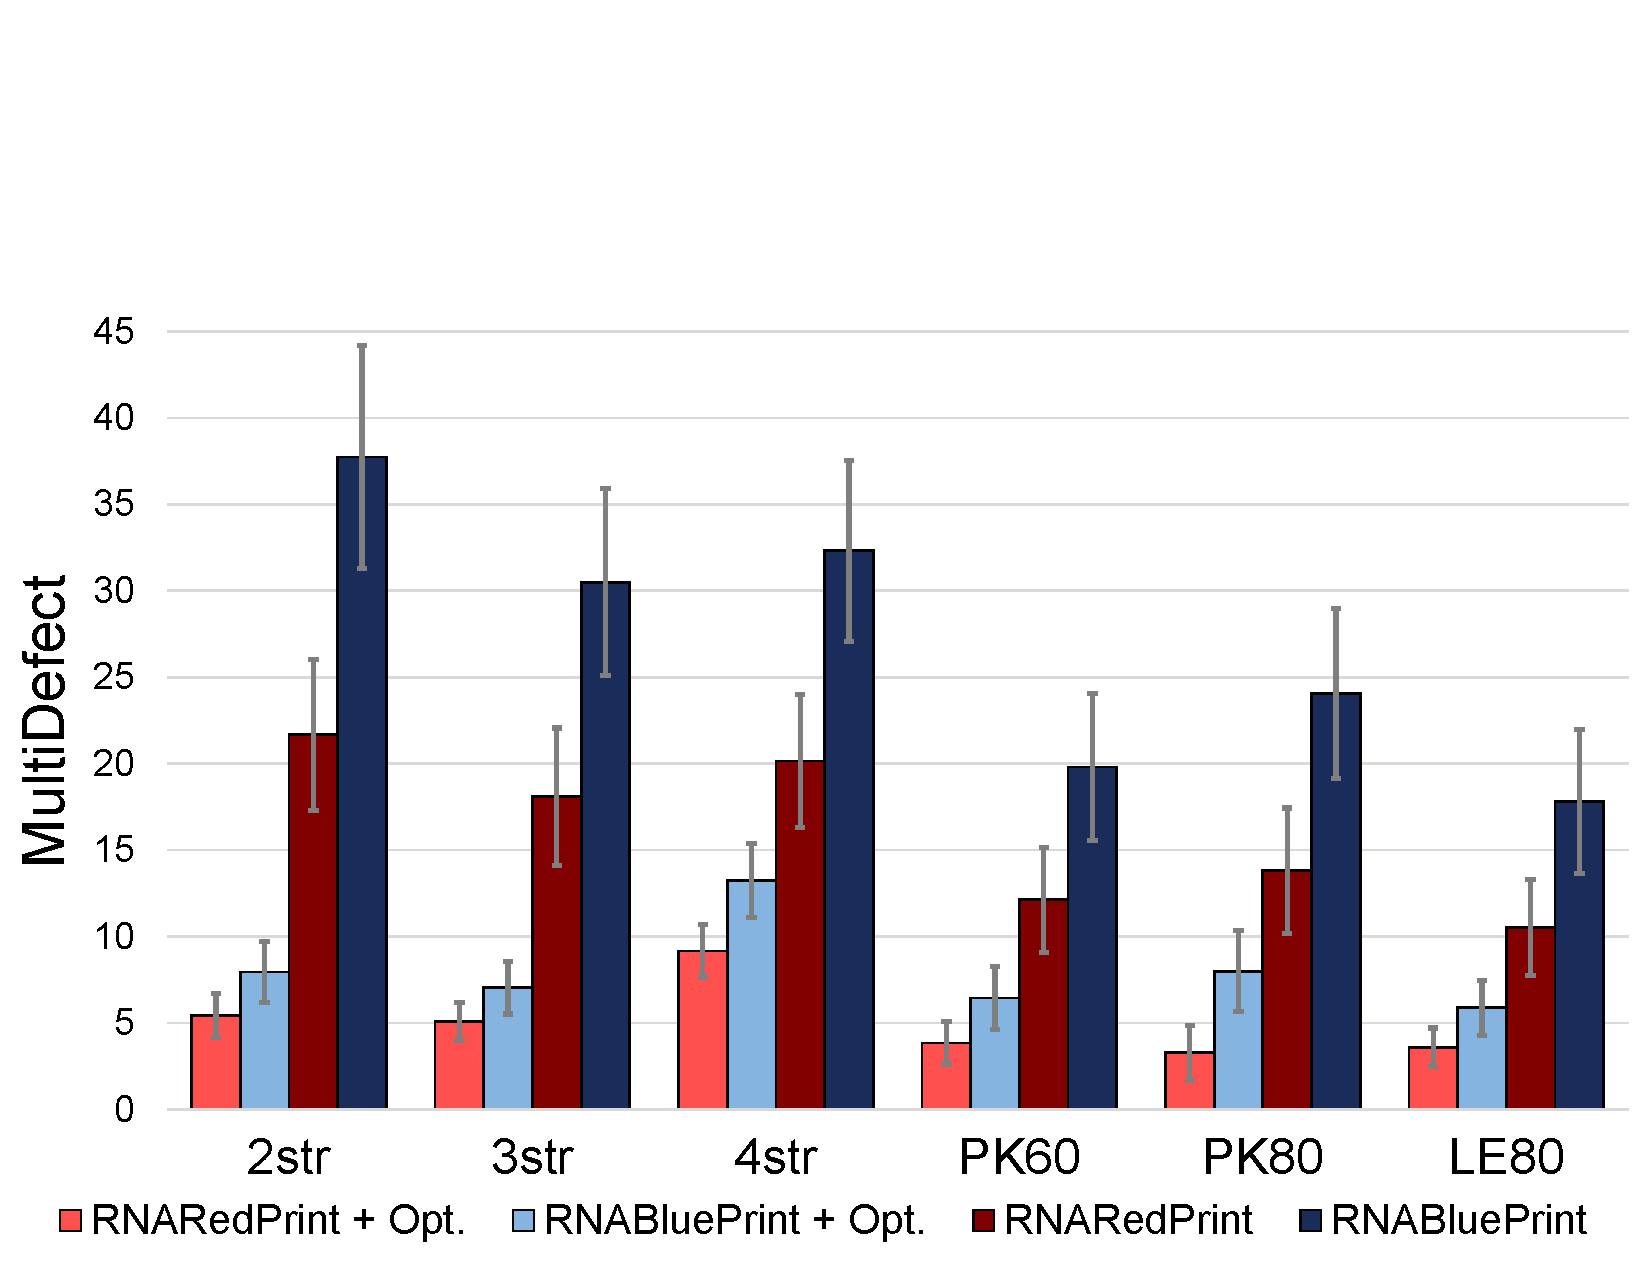
\includegraphics[width=.9\linewidth,trim={.2cm .3cm .2cm 5cm},clip]{Figs/statistics-overall}}
  \caption{Comparison of the \Obj{} (see
    Eq.~\eqref{eq:blueprintobjective}; smaller values $\to$ better
    designs) for sequences sampled by \ourprog{} and uniform sampling
    (\RNAblueprint) for six benchmark sets. For both sampling schemes,
    we show the MultiDefects of the sampled sequences, as well as
    results after further optimization by local search (``+ Opt.'').}
\label{fig:benchmark-results}
\end{figure}

\section{\#{\sf P}-hardness of counting valid designs}\label{sec:counting}
%%% reformulate later
%We define the following notations: $\real^\infty:=\real\cup\{\infty\}$, $[i,j]:=\{i,\ldots,j\},$ \ldots
Finally, we turn to the complexity of $\NumDesign(G)$, the problem of
computing the number of valid sequences for a given compatibility
graph $G=(V,E)$. Note that this problem corresponds to the partition
function problem in a simple base pair model, assigning $0$ to
canonical and $\infty$ to non-canonical base pairs and setting
$\beta>0$, so that any valid structure counts as $1$ in the partition
function. As previously noted~\citep{Flamm2001}, a set of target
structures admits a valid design iff its compatibility graph is
bipartite, which can be tested in linear time.  Moreover, without
$\{\Gb, \Ub\}$ base pairs, the design of any connected component $C$
of $G$ would be entirely determined by the assignment of a single of
its nucleotides. The number of valid designs is thus simply
$4^{\#{\rm CC}(G)}$, where $\#{\rm CC}(G)$ is the \Def{number of
  connected components}.

The problem becomes much harder when $\{\Gb, \Ub\}$ base pairs are allowed, and we show that valid designs for a set of structures cannot be counted in polynomial time, unless ${\sf\# P}={\sf FP}$. This equality would, in particular, imply the classic ${\sf P}={\sf NP}$.

To establish that claim, we consider instances $G=(V_1\cup V_2, E)$ that are connected and bipartite ($E \cap (V_1\times V_2) = E$), noting that hardness over restricted instances implies hardness of the general problem. Moreover note that, as observed in Subsec.~\ref{sec:complexity}, assigning a nucleotide to a position $u\in V$ constrains the parity ($\{\Ab,\Gb\}$ or $\{\Cb,\Ub\}$) of all positions in the connected component of $u$. For this reason, we restrict our attention to the counting of valid designs \emph{up to trivial  symmetry} $(\Ab\leftrightarrow \Cb/\Gb\leftrightarrow \Ub)$, by constraining the positions in $V_{1}$ to $\Ab$ and $\Gb$. Let $\Design{G}$ denote the subset of all designs for $G$ under this constraint, noting that $\NumDesign(G) = 2\cdot|\Design{G}|$.

Let $\IS{G}$ denote the set of all independent sets in the connected graph $G$; recall that an \Def{independent set} of $G=(V,E)$ is a subset $V'\subseteq V$ of nodes that are not connected by any edge in $E$. 

\begin{proposition}
  $\Design{G}$ and $\IS{G}$ have equal size.
\end{proposition}
%
\begin{proof}
Consider $\Psi: \Design{G} \to \IS{G}$ defined by $ \Psi(f) := \left\{v\in V\mid f(v)\in\{\Ab,\Cb\}\right\}.$
We show that $\Psi$ is bijective:%
\begin{itemize}
\item $\Psi$ is injective, i.e. $\Psi(f)\neq\Psi(f')$ for all $f\neq f'$.
If $f\neq f'$, then there exists a node $v\in V$ such that $f(v)\neq f'(v)$.
We discuss only the case $v\in V_1$, where we restricted the nucleotides to $\Ab$ and $\Gb$. Then, $\{f(v),f'(v)\}$ must equal $\{\Ab,\Gb\}$, such that either $v\in\Psi(f)$ or $v\in\Psi(f')$.
%
\item $\Psi$ is surjective, i.e. there is a preimage for each element $I\in \IS{G}$. Define $f\in\Design{G}$ as\begin{displaymath}
f(v) = \left\{\begin{array}{ll@{\qquad}ll}
\Ab{} & \text{if $v\in V_1$ and $v\in I$} &
\Cb{} & \text{if $v\in V_2$ and $v\in I$}\\
\Gb{} & \text{if $v\in V_1$ and $v\not\in I$} &
\Ub{} & \text{if $v\in V_2$ and $v\not\in I$}
\end{array}\right.
\end{displaymath}
One easily verifies that $\Psi(f) = I$.
%
%for any $(v_1,v_2)\in V_1\times V_2$ by
%\begin{align*}
%f(v_1) &= \begin{cases} \Ab & \text{if }v_1\in S\\ \Gb & \text{if }v_1\notin S\end{cases} &
%\text{\quad and\quad}&&
% f(v_2) &= \begin{cases} \Cb & \text{if }v_2\in S\\ \Ub & \text{if }v_2\notin S.\end{cases}
%\end{align*}
%
It remains to show that $f$ is a valid design for $G$, i.e. for each $(v, v') \in E$, $\{f(v),f(v')\}\in \B$; please recall that we defined $\B$ as the set of all valid nucleotide pairs.
Assume there is an edge $(v_1,v_2)\in E$, violating $\{f(v_1),f(v_2)\} \in \B$. Since $G$ is bipartite,
$v_1\in V_1$ and $v_2\in V_2$, such that $f(v_1)\in\{\Ab,\Gb\}$ and $f(v_2)\in\{\Cb,\Ub\}$. This implies that among all possible $\{f(v_1), f(v_2)\}$ only $\{\Ab,\Cb\}$ is not in $\B$, which in turn requires $v_1\in I$ and $v_2\in I$. Therefore, since $I$ is an independent set, the edge $(v_1,v_2)\in E$ cannot exist. 
\end{itemize}
\end{proof}

Now we can build on the connection between the two problems to obtain complexity results for \NumDesign. Counting independent sets in bipartite graphs ($\#{\sf BIS}$) is indeed a well-studied \#{\sf P}-hard problem~\citep{Ge2012}, from which we immediately conclude:
\begin{corollary}
  \NumDesign is $\#{\sf P}$-hard
\end{corollary}
\begin{proof}
  Note that $\#{\sf BIS}$ is also \#{\sf P}-hard on connected graphs, as the number of independent sets for a disconnected graph $G$ is given by $|\IS{G}|=\prod_{cc\in CC(G)} |\IS{cc}|$. Thus any efficient algorithm for $\#{\sf BIS}$ on connected instances provides an efficient algorithm for general graphs.

  Let us now hypothesize the existence of a polynomial-time algorithm $\mathcal{A}$ for \NumDesign over strongly-connected graphs $G$. Consider the (polynomial-time) algorithm $\mathcal{A}'$ that first executes $\mathcal{A}$ on $G$ to produce $\NumDesign(G)$, and returns $\NumDesign(G)/2=|\Design{G}| = |\IS{G}|$. Clearly $\mathcal{A}'$ solves $\#{\sf BIS}$ in polynomial-time. This means that $\NumDesign$  is at least as hard as $\#{\sf BIS}$, thus does not admit a polynomial time exact algorithm unless $\#{\sf P}={\sf FP}$.
\end{proof}

\section{Conclusion}
Motivated by the---here established---hardness of the problem, we
introduced a general framework, and efficient algorithms to design RNA
sequences that may adopt multiple target structures with fine-tuned
properties. Our method combines an FPT stochastic sampling algorithm
with multi-dimensional Boltzmann sampling over distributions
controlled by expressive RNA energy models.  Compared to the
previously best available sampling method (uniform sampling), this
approach generated significantly better seed sequences for instances
of an extensive multi-target design benchmark, including pseudoknots.

The presented method enables new possibilities for the sequence generation
in the field of RNA sequence design, allowing to enforce additional
constraints, like \GCb\%, while controlling the energy of
multiple target structures. Thus it presents a major advance over
previously applied ad-hoc sampling and even efficient uniform sampling
strategies. We have shown the practicality of such controlled sequence
generation, including the case of pseudoknotted structures, and studied its use for multi-target RNA design. Moreover,
our framework is amenable to extensions, to include more complex sequence
constraints, including mandatory/forbidden motifs at specific
positions, or anywhere in the designed sequences, by adapting formal language constructs
introduced by \citet{Zhou2013}. Negative design principles could also
be explicitly supported at the generation stage, for instance by
penalizing a set of alternative helices/structures.


%%%%%%%%%%%%%%%%%%%%%%%%%%%%%%%%%%%%%%%%%%%%%%
%%                                          %%
%% Backmatter begins here                   %%
%%                                          %%
%%%%%%%%%%%%%%%%%%%%%%%%%%%%%%%%%%%%%%%%%%%%%%

\begin{backmatter}

\section*{Competing interests}
  The authors declare that they have no competing interests.

\section*{Author's contributions}
  All authors wrote the manuscript.
    % Text for this section \ldots
    % http://www.biomedcentral.com/submissions/editorial-policies\#authorship

\section*{Acknowledgements}
YP is supported
%jointly supported
by the
% French
{\em Agence
  Nationale de la Recherche} and the
%Austrian
FWF (ANR-14-CE34-0011; project RNALands).  SH is supported by the
German Federal Ministry of Education and Research (BMBF support code
031A538B; de.NBI: German Network for Bioinformatics Infrastructure)
and the
% acknowledged by
%financial support of the
Future and Emerging Technologies programme
% within the Seventh Framework Programme for Research of the
%European Commission, under
(FET-Open grant 323987; project RiboNets).
%
We thank Leonid Chindelevitch for suggesting a drastic optimization of our FPT algorithm based on stable sets combinatorics, and Arie Koster for practical recommendations on tree decompositions.

%%%%%%%%%%%%%%%%%%%%%%%%%%%%%%%%%%%%%%%%%%%%%%%%%%%%%%%%%%%%%
%%                  The Bibliography                       %%
%%                                                         %%
%%  Bmc_mathpys.bst  will be used to                       %%
%%  create a .BBL file for submission.                     %%
%%  After submission of the .TEX file,                     %%
%%  you will be prompted to submit your .BBL file.         %%
%%                                                         %%
%%                                                         %%
%%  Note that the displayed Bibliography will not          %%
%%  necessarily be rendered by Latex exactly as specified  %%
%%  in the online Instructions for Authors.                %%
%%                                                         %%
%%%%%%%%%%%%%%%%%%%%%%%%%%%%%%%%%%%%%%%%%%%%%%%%%%%%%%%%%%%%%

% if your bibliography is in bibtex format, use those commands:
\bibliographystyle{bmc-mathphys} % Style BST file (bmc-mathphys, vancouver, spbasic).
\bibliography{biblio}      % Bibliography file (usually '*.bib' )
% for author-year bibliography (bmc-mathphys or spbasic)
% a) write to bib file (bmc-mathphys only)
% @settings{label, options="nameyear"}
% b) uncomment next line
%\nocite{label}

% or include bibliography directly:
% \begin{thebibliography}
% \bibitem{b1}
% \end{thebibliography}

%%%%%%%%%%%%%%%%%%%%%%%%%%%%%%%%%%%
%%                               %%
%% Figures                       %%
%%                               %%
%% NB: this is for captions and  %%
%% Titles. All graphics must be  %%
%% submitted separately and NOT  %%
%% included in the Tex document  %%
%%                               %%
%%%%%%%%%%%%%%%%%%%%%%%%%%%%%%%%%%%

%%
%% Do not use \listoffigures as most will included as separate files

 \section*{Figures}
%   \begin{figure}[h!]
%   \caption{\csentence{Sample figure title.}
%       A short description of the figure content
%       should go here.}
%       \end{figure}
% 
% \begin{figure}[h!]
%   \caption{\csentence{Sample figure title.}
%       Figure legend text.}
%       \end{figure}

%%%%%%%%%%%%%%%%%%%%%%%%%%%%%%%%%%%
%%                               %%
%% Tables                        %%
%%                               %%
%%%%%%%%%%%%%%%%%%%%%%%%%%%%%%%%%%%

%% Use of \listoftables is discouraged.
%%
% \section*{Tables}
% \begin{table}[h!]
% \caption{Sample table title. This is where the description of the table should go.}
%       \begin{tabular}{cccc}
%         \hline
%            & B1  &B2   & B3\\ \hline
%         A1 & 0.1 & 0.2 & 0.3\\
%         A2 & ... & ..  & .\\
%         A3 & ..  & .   & .\\ \hline
%       \end{tabular}
% \end{table}

%%%%%%%%%%%%%%%%%%%%%%%%%%%%%%%%%%%
%%                               %%
%% Additional Files              %%
%%                               %%
%%%%%%%%%%%%%%%%%%%%%%%%%%%%%%%%%%%

% \section*{Additional Files}
%   \subsection*{Additional file 1 --- Sample additional file title}
%     Additional file descriptions text (including details of how to
%     view the file, if it is in a non-standard format or the file extension).  This might
%     refer to a multi-page table or a figure.
%
%  \subsection*{Additional file 2 --- Sample additional file title}
%    Additional file descriptions text.


\end{backmatter}
\end{document}
